% !TEX root = ../my_thesis.tex

\section{Ergebnisse}
 \label{sec:kapitel_4}

Im vorliegenden Kapitel werden die Ergebnisse der durchgeführten Experimente präsentiert. Ein Evaluationsergebnis gibt in dieser Arbeit die Abweichung der Position in Metern und den Orientierungsfehler in Grad an. Ferner wird ein Evaluationsergebnis gegenüber Seinesgleichen anhand seines Positionsfehlers verglichen. Außerdem wird die Akkuratesse eines KNNs durch den Median aller Evaluationsergebnisse bestimmt. Im weiteren Verlauf dieses Kapitels werden zuerst die Reproduktionsergebnisse von BIM-PoseNet \cite{acharyaBIMPoseNetIndoorCamera2019} angegeben und danach die Evaluationsergebnisse der trainierten Netzwerke dargestellt.

\subsection{Reproduktion der Ergebnisse von BIM-PoseNet}
Die Ergebnisse der Experimente von \citet{acharyaBIMPoseNetIndoorCamera2019} (\textit{BIM-PoseNet}), die das PoseNet Model mit den Gradientenbildern der karikaturistischen Daten (\textit{grad-cartoon}) sowie synthetischen Kantenbilder trainierten (\textit{grad-edge}) und anschließend mit den Gradientenbildern der realen Daten (\textit{grad-real}) evaluierten, konnten näherungsweise reproduziert werden (vgl. Tab. \ref{tab:reproduction}). Abweichend von BIM-PoseNet wurden statt 1000 \textit{grad-real} Daten, 600 \textit{grad-real} Daten evaluiert, weil zu derzeit 600 Evaluierungsbilder veröffentlicht waren. Der Trainingsprozess wurde pro Datensatztyp 5-mal wiederholt und die bessere Akkuratesse wurde behalten. Eine exakte oder bessere Reproduktion der Ergebnisse ist durch Zufall bedingt und wurde in dieser Arbeit aus Zeitgründen vernachlässigt. Tabelle \ref{tab:reproduction} präsentiert die Ergebnisse der Reproduktion.


\begin{table}[b]
	\centering
	\caption{Reproduktionsergebnisse. Abweichungen der Ergebnisse sind durch Zufall bedingt und können bei mehrfachem Wiederholen des Trainingsprozesses minimiert bzw. erhoben sowie verbessert werden. }
	\begin{tabularx}{1.0\textwidth}{X X X}
		\textbf{Netzwerk} \hspace{2cm} (Trainingsdatensatz) & \textbf{BIM-PoseNet} \hspace{2cm} (Position, Orientierung) & \textbf{Reproduktion} \hspace{2cm} (Position, Orientierung)\\
		\hline
	 \textit{grad-cartoon} & 2.63$m$, 6.99° & 2.57$m$, 10.52°\\
		\hline
		\textit{grad-edge} & 1.88$m$, 7.73° & 2.53$m$, 9.54°\\
	\end{tabularx}
	\label{tab:reproduction}
\end{table}





\subsection{Evaluation der trainierten KNNs}
Für alle synthetischen Datensätze wurde das Trainingsprozess 5-mal mit den korrespondierenden Gradientenbildern der Trainingsdaten separat wiederholt. Eine Evaluierung folgte mit den Gradientenbildern der korrespondierenden synthetischen und realen Evaluationsdaten. Es wurden pro Strecke je Datensatztyp nur die beste Akkuratesse behalten. Tabelle \ref{tab:results_ic} bis \ref{tab:results_hs_stairs_down} geben die Akkuratesse der KNNs auf den jeweiligen Strecken an. 

Für ein besseres Verständnis der durch die Evaluierung mit den \textit{grad-real} Datensätzen resultierenden Akkuratesse wurden pro Strecke für die besten Netzwerke die bestimmten Positionen in der xy-Ebene dargestellt. Ebenso wurden pro Strecke die Positionsfehler in der xy-Ebene und die Orientierungsfehler auf der Gierachse der jeweiligen Evaluationsdaten dargestellt. Abbildungen \ref{fig:result_ic_loop} bis \ref{fig:result_hs_stairs_down} illustrieren die Evaluationsergebnisse.


\subsubsection{IC-loop}
\label{subsubsec:ic_loop}
% die eine geschlossen Schleife in einem optisch ähnlichen Flur bildet,
% der Ansatz von \citet{acharyaBIMPoseNetIndoorCamera2019} auf einer ebenen, gegen den UZS abwechselnde Richtung verlaufenden, ca. 115$m$ langen Strecke mit wiederholenden Gebäudemerkmalen 
% Alle Datensätze der Strecke \textit{IC-loop} wurden zu 50\% Trainingsdaten und zu 50\% Evaluierungsdaten zufällig aufgeteilt. Für alle synthetischen Datensatztypen mit je 5718 Daten wurde ein separates Netzwerk trainiert. Anschließend wurden die Netzwerke mit den korrespondierenden synthetischen Evaluierungsdatensätze mit je 5717 Daten getestet. Eine weitere Evaluierung der trainierten Netzwerke folgte mit den realen 1921 Evaluierungsdaten. Tabelle \ref{tab:results_ic} gibt die Ergebnisse dieser Evaluierungsvorgänge an.
% Aus Tabelle \ref{tab:results_ic} ist zu erkennen,
% Dies zeigt die potenzielle Fähigkeit des Experimentes zur Pose Bestimmung mit Daten derselben Domäne auf der \textit{IC-loop} Strecke. 

In diesem Experiment wurde der \textit{IC-loop} Datensatz verwendet. 
Eine Akkuratesse von 1.61$m$ in der Position und 8.17° in der Orientierung wurde ausschließlich mit synthetischen Daten beim Trainieren und Evaluieren durch den \textit{grad-cartoon} Datensatz erzielt. Bei der Evaluierung mit den Gradientenbildern der realen Evaluationsdaten wurde auf dem \textit{grad-photoreal} Netzwerk eine Akkuratesse von 16.68$m$ in der Position und 73.25° in der Orientierung erreicht (vgl. Tab. \ref{tab:results_ic}). 

% Bei einem Gebäudevolumen von ca. $50m \times 11m \times 3.5m$ ist die Positionsgenauigkeit von 16.68$m$, mit Anbetracht des Abdriftens der realen Ground-Truth-Daten (s. Abschn. \ref{subsec:record_real_data}), für ein denkbares Lokalisierungsverfahren zu ungenau. Genauso ist eine Orientierungsgenauigkeit von 73.25° für die Bestimmung der Orientierung mehr als ungeeignet. Abbildung \ref{fig:result_ic_loop} visualisiert die Evaluierungsergebnisse von dem mit \textit{grad-photoreal} trainiertem sowie mit \textit{grad-real} evaluiertem Netzwerk.

Das \textit{grad-photoreal} Netzwerk bestimmte nur die Positionen aller \textit{grad-real} Evaluationsdaten auf einem ca. $30m \times 5m$ großen Teilbereich der unteren horizontalen Strecke (vgl. Abb. \ref{subfig:ic_fig2}). Daher wiesen Evaluationsdaten der kürzeren vertikalen sowie der obigen horizontalen Strecke die größten Positionsfehler auf (vgl. Abb. \ref{subfig:ic_fig4}). Ebenso bestimmte das Netzwerk größtenteils die Orientierung der Evaluationsdaten als die Aufnahmerichtung der unteren horizontalen Strecke (vgl. Abb. \ref{subfig:ic_fig6}).

\begin{table}
	\centering
	\caption{Evaluationsergebnisse von der Strecke \textit{IC-loop}. Die Akkuratesse der mit den jeweiligen Trainingsdaten trainierten Netzwerken wird angegeben. Diese Netzwerke wurde mit den korrespondierenden synthetischen Evaluationsdaten und jeweils mit den realen Evaluationsdaten evaluiert.}
	\begin{tabularx}{1.0\textwidth}{X >{\RaggedRight}X >{\RaggedRight}X}
	\textbf{Trainingsdatensatz} \hspace{2cm} (Gradientenbild) & \textbf{synthetische Daten} \hspace{2cm} (Position, Orientierung) & \textbf{reale Daten} \hspace{2cm} (Position, Orientierung)\\
	\hline
		\textit{grad-cartoon} & 1.61$m$, 8.17° & 23.56$m$, 51.30°\\
		\hline
		\textit{grad-edge} & 2.00$m$, 8.29° & 32.91$m$, 59.17°\\
		\hline
		\textit{grad-photoreal} & 1.80$m$, 7.70° & 16.68$m$, 73.25°\\
		\hhline
		Durschnitt & 1.80$m$, 7.70° & 16.68$m$, 73.25°\\
	\end{tabularx}
	\label{tab:results_ic}
\end{table}



\begin{figure}
	\setlength\extrarowheight{-15pt}
	\centering
	\begin{tabularx}{0.9\textwidth}{>{\centering\arraybackslash}p{0.05\textwidth} X}
		\subcaption{} \label{subfig:ic_fig2} & \imagetop{ 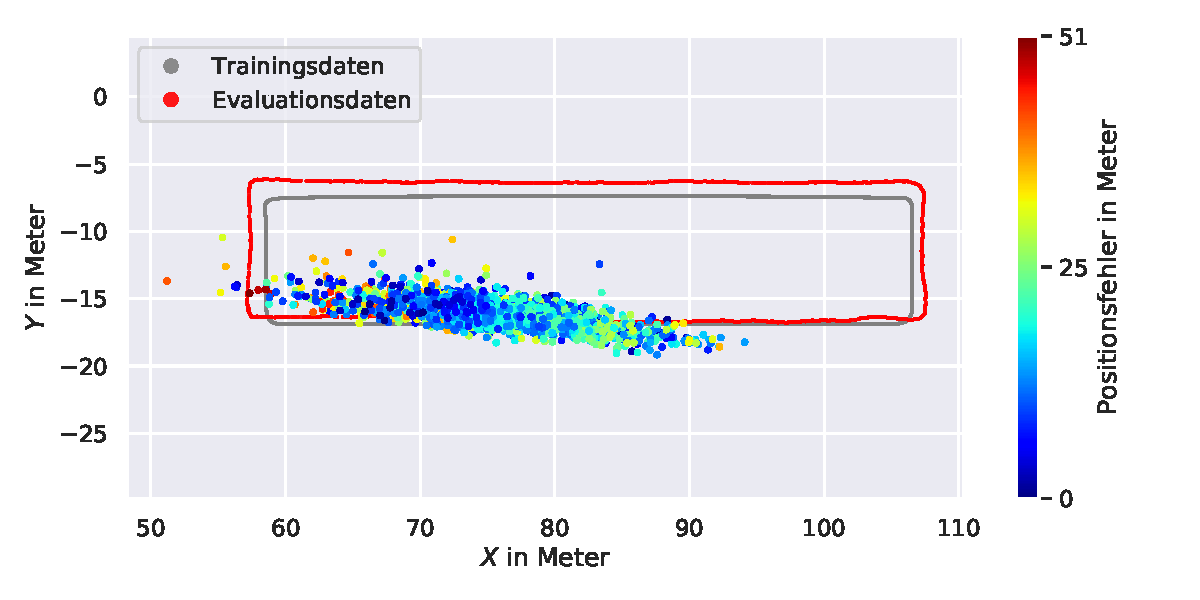
\includegraphics[width=1.0\linewidth]{images/results/ic_cycl/resultsfig_2.pdf} }\\
		\subcaption{} \label{subfig:ic_fig4} & \imagetop{ 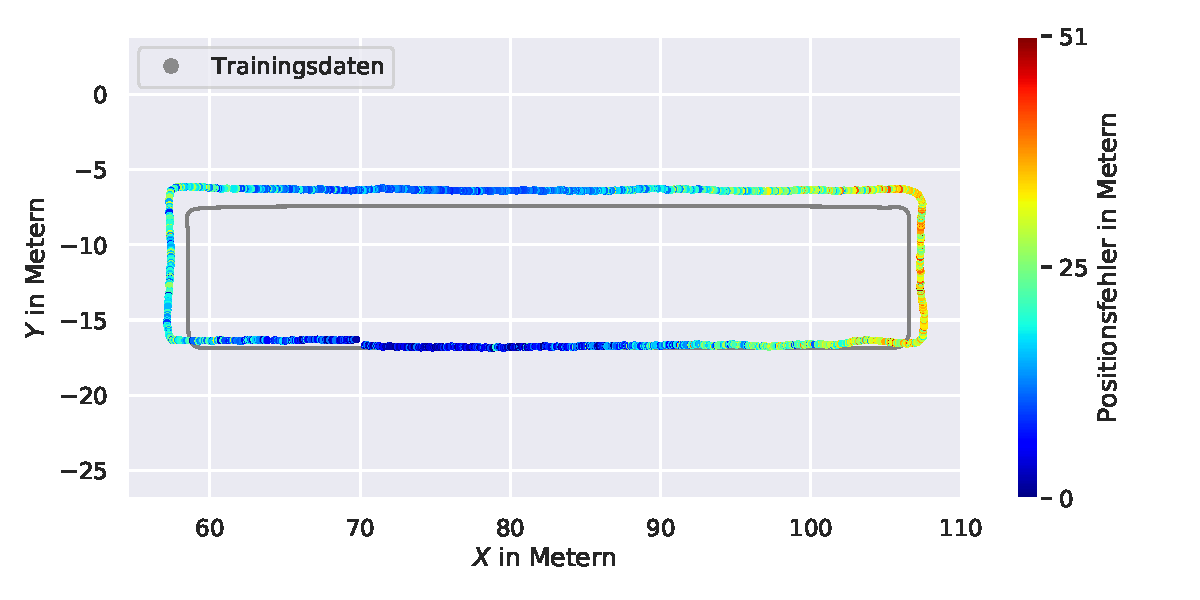
\includegraphics[width=1.0\linewidth]{images/results/ic_cycl/resultsfig_4.pdf} }\\
		\subcaption{} \label{subfig:ic_fig6} & \imagetop{ 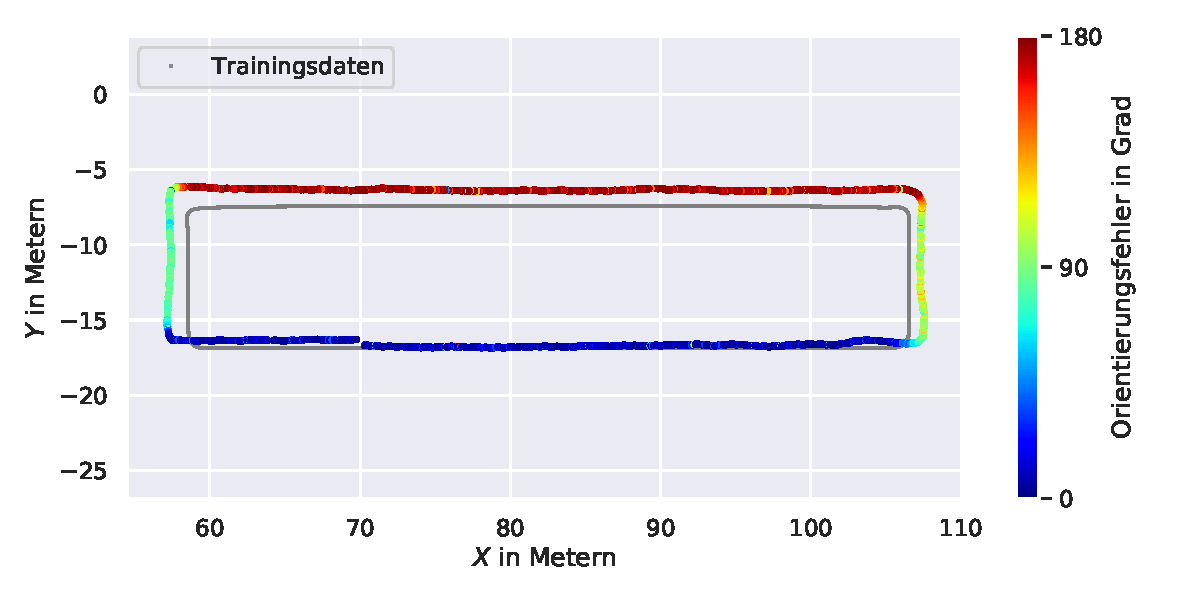
\includegraphics[width=1.0\linewidth]{images/results/ic_cycl/resultsfig_6.pdf} }\\
	\end{tabularx}
	\caption{Visualisierung der Evaluationsergebnisse der Strecke \textit{IC-loop} (s. Abb. \ref{subfig:traj_ic}). Die Evaluation folgte mit den Gradietenbildern der realen Daten auf dem mit \textit{grad-photoreal} trainierten Netzwerk. \subref{subfig:ic_fig2} illustriert die von dem KNN bestimmten Positionen auf der xy-Ebene. Der Positionsfehler in der xy-Ebene und der Orientierungsfehler auf der Gierachse der jeweiligen Evaluationsdaten werden in \subref{subfig:ic_fig4} und \subref{subfig:ic_fig6} dargestellt.}
	\label{fig:result_ic_loop}
\end{figure}


\subsubsection{HS-gamma}
\label{subsubsec:hs_gamma}
%Dies stellt bei dem betroffenen Gebäudevolumen von $54m \times 10m \times 3m$ ein Potenzial zur Pose Estimation mit Daten der gleichen Beschaffenheit dar.
Ein weiteres Experiment folgte mit dem \textit{HS-gamma} Datensatz. Trainiert und evaluiert mit nur synthetischen Daten wurde durch den \textit{grad-cartoon} Datensatz eine Akkuratesse von 1.00$m$ in der Position und 9.92° in der Orientierung erzielt. Die Evaluierung mit den \textit{grad-real} Evaluationsdaten auf dem \textit{grad-cartoon} Netzwerk führte zur einer Akkuratesse von 8.60$m$ in der Position und 19.59° in der Orientierung (vgl. Tab. \ref{tab:results_hs_gamma}). 

% Bei oben genannten Gebäudemaßen ist eine Positionsgenauigkeit von 8.60$m$ sowie ein Orientierungsfehler von 19.59° unzureichend für die Bestimmung der Pose auf der \textit{HS-gamma} Strecke. Abbildung \ref{fig:result_hs_gamma} visualisiert die Evaluationsergebnisse von dem mit \textit{grad-cartoon} trainiertem und \textit{grad-real} evaluiertem Netzwerk.

Das \textit{grad-cartoon} Netzwerk bestimmte überwiegend die Positionen aller \textit{grad-real} Evaluationsdaten auf der linken horizontalen Strecke auf einem ca. $20m \times 5m$ großen Teilbereich (vgl. Abb. \ref{subfig:hs_gamma_fig2}). Deshalb wiesen die Evaluationsdaten der linken horizontalen Strecke die geringsten Positionsfehler auf. Zudem zeigten die Evaluationsdaten des zum Ausgangspunkt optisch ähnlichen Flures die größten Positionsfehler auf (vgl. Abb. \ref{subfig:ic_fig4}). Ebenso bestimmte das oben erwähnte Netzwerk mehrheitlich die Orientierung der Evaluationsdaten als die Orientierung der dominierenden Aufnahmerichtung. Daher waren die größten Orientierungsfehler bei den Evaluationsdaten der Schlaufe sowie der vertikal verlaufenden Strecke aufzufinden (vgl. Abb. \ref{subfig:ic_fig4}). 


\begin{table}
	\centering
	\caption{Evaluationsergebnisse von der Strecke \textit{HS-gamma}. Die Akkuratesse der mit den jeweiligen Trainingsdaten trainierten Netzwerken wird angegeben. Diese Netzwerke wurde mit den korrespondierenden synthetischen Evaluationsdaten und jeweils mit den realen Evaluationsdaten evaluiert.}
	\begin{tabularx}{1.0\textwidth}{X >{\RaggedRight}X >{\RaggedRight}X}
		\textbf{Netzwerk} \hspace{2cm} (Trainingsdatensatz) & \textbf{synthetische Daten} \hspace{2cm} (Position, Orientierung) & \textbf{reale Daten} \hspace{2cm} (Position, Orientierung)\\
	\hline
		\textit{grad-cartoon} & 1.00$m$, 9.92° & 8.60$m$, 19.59°\\
		\hline
		\textit{grad-edge} & 1.07$m$, 8.69° & 10.15$m$, 35.11°\\
		\hline
		\textit{grad-photoreal} & 1.45$m$, 9.17° & 10.27$m$, 41.60°\\
	\end{tabularx}
	\label{tab:results_hs_gamma}
\end{table}

\begin{figure}
	\setlength\extrarowheight{-15pt}
	\centering
	\begin{tabularx}{0.9\textwidth}{>{\centering\arraybackslash}p{0.05\textwidth} X}
		\subcaption{} \label{subfig:hs_gamma_fig2} & \imagetop{ 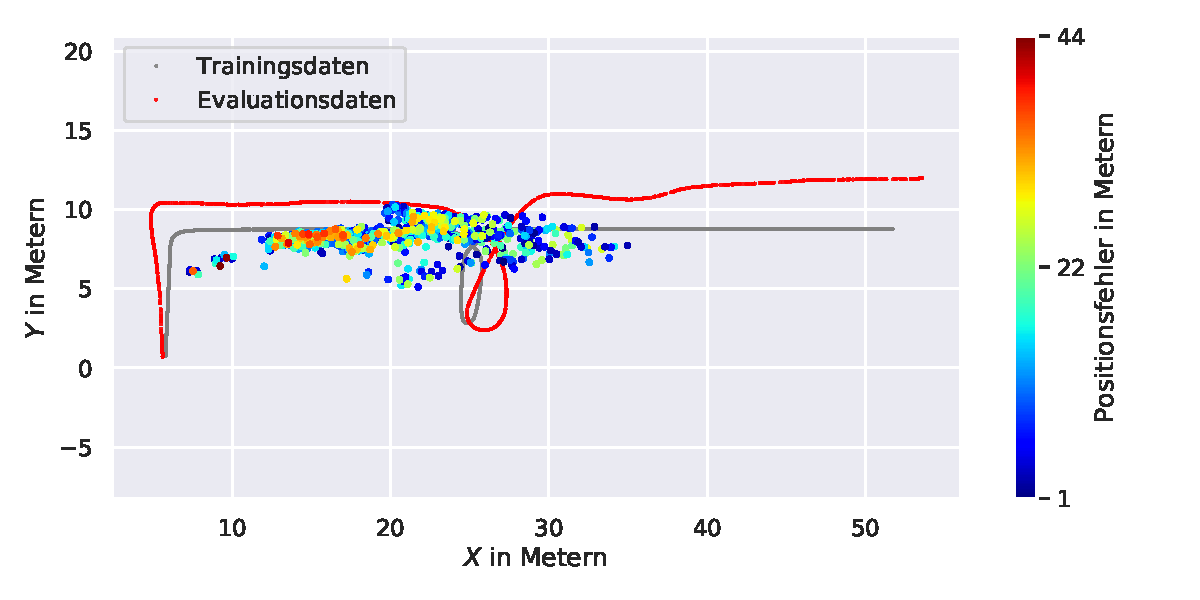
\includegraphics[width=1.0\linewidth]{images/results/hs_gamma/resultsfig_2.pdf} }\\
		\subcaption{} \label{subfig:hs_gamma_fig4} & \imagetop{ 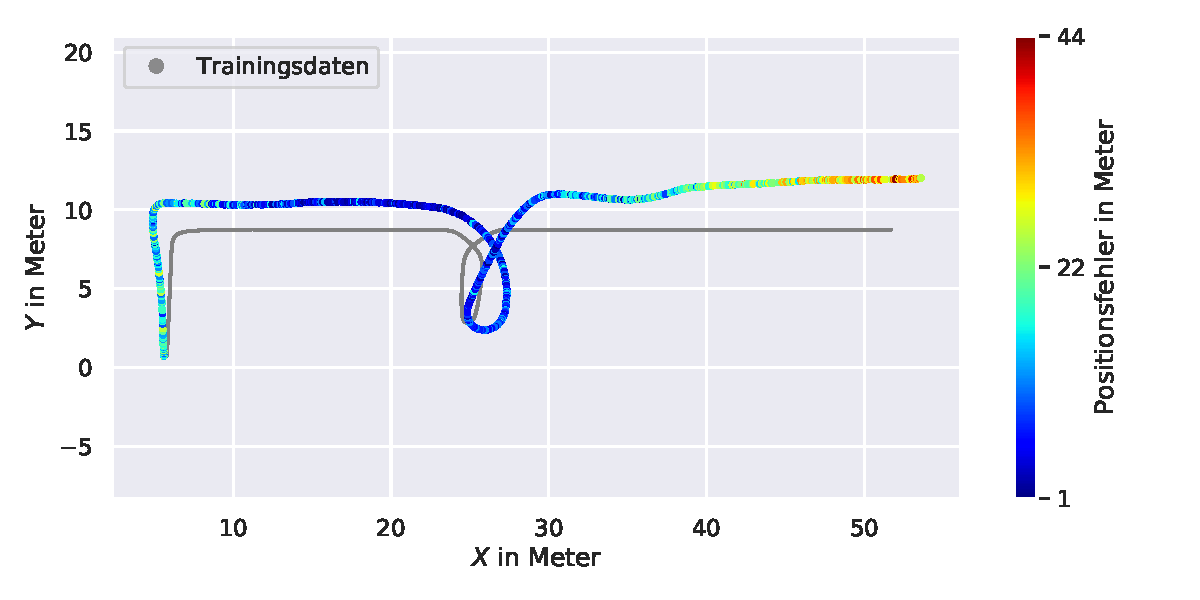
\includegraphics[width=1.0\linewidth]{images/results/hs_gamma/resultsfig_4.pdf} }\\
		\subcaption{} \label{subfig:hs_gamma_fig6} & \imagetop{ 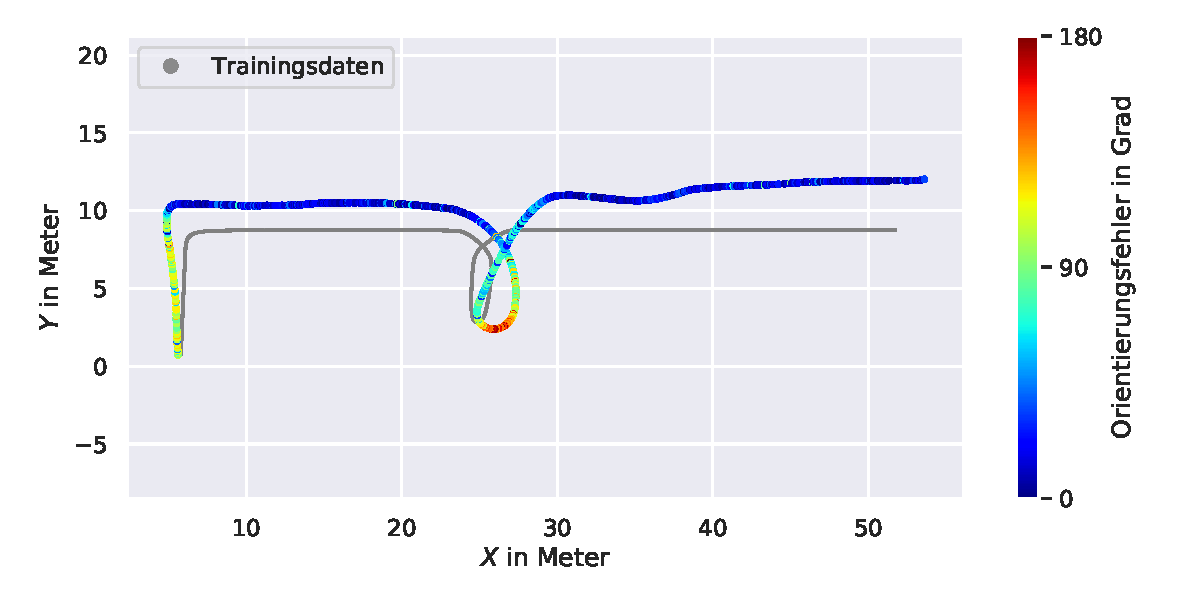
\includegraphics[width=1.0\linewidth]{images/results/hs_gamma/resultsfig_6.pdf} }\\
	\end{tabularx}
	\caption{Visualisierung der Evaluationsergebnisse der Strecke \textit{HS-gamma} (s. Abb. \ref{subfig:traj_hs_gamma}). Die Evaluation folgte mit den Gradietenbildern der realen Daten auf dem mit \textit{grad-cartoon} trainierten Netzwerk. \subref{subfig:hs_gamma_fig2}  illustriert die von dem KNN bestimmten Positionen auf der xy-Ebene. Der Positionsfehler der xy-Ebene und der Orientierungsfehler auf der Gierachse der jeweiligen Evaluationsdaten werden in \subref{subfig:hs_gamma_fig4} und \subref{subfig:hs_gamma_fig6} dargestellt.}
	\label{fig:result_hs_gamma}
\end{figure}

\subsubsection{HS-stairs-up}
\label{subsubsec:hs_stairs_up}
% Dies zeigt das Potenzial des Experimentes zur Pose Bestimmung mit Daten derselben Domäne auf der \textit{HS-stairs-up} Strecke.

Weiterhin wurde ein Experiment mit dem \textit{HS-stairs-up} Datensatz durchgeführt. Ausschließlich mit synthetischen Daten wurde eine Akkuratesse von 0.82$m$ in der Position und 7.76° in der Orientierung durch die \textit{grad-cartoon} Daten erzielt. Bei der Evaluierung mit den Gradientenbildern der realen Evaluationsdaten wurde eine Akkuratesse von 4.33$m$ in der Position und 51.64° in der Orientierung durch das \textit{grad-edge} Netzwerk erreicht (vgl. Tab. \ref{tab:results_hs_stairs_up}). 

% Sowohl ein Positionsfehler von 4.33$m$ als auch ein Orientierungsfehler von 51.64° sind für die Bestimmung der Pose auf der \textit{HS-stairs-up} Strecke in einem ca. $12m \times 12m \times 12m$ großen Zone ungenügend. Abbildung \ref{fig:result_hs_stairs_up} visualisiert die Evaluationsergebnisse von dem mit \textit{grad-edge} trainiertem und \textit{grad-real} evaluiertem Netzwerk.

Die vom \textit{grad-edge} Netzwerk bestimmten Positionen aller \textit{grad-real} Evaluationsdaten liegen mehrheitlich zwischen dem unteren und oberen Treppenlauf (vgl. Abb. \ref{subfig:hs_up_fig3}). Deshalb waren die größten Positionsfehler bei den Evaluationsdaten des Treppenabsatzes aufzufinden. Ebenso waren bei den Evaluationsdaten des unteren und oberen Treppenlaufes abwechselnd größere Positionsfehler zu erkennen. Hierbei weisten die Evaluationsdaten des oberen Treppenlaufes häufiger einen größeren Positionsfehler auf (vgl. Abb. \ref{subfig:hs_up_fig5}). Die Orientierung der Evaluationsdaten des oberen Treppenlaufes wurden überwiegend als die Orientierung der Evaluationsdaten des unteren Treppenlaufes bestimmt. Ebenso waren bei den Evaluationsdaten der Treppenläufe abwechselnd in der entgegengesetzten Orientierung Fehler zu erkennen (vgl. Abb. \ref{subfig:hs_up_fig7}).

\begin{table}
	\centering
	\caption{Evaluationsergebnisse von der Strecke \textit{HS-stairs-up} (s. Abb. \ref{subfig:traj_hs-up}). Die Akkuratesse der mit den jeweiligen Trainingsdaten trainierten Netzwerken wird angegeben. Diese Netzwerke wurde mit den korrespondierenden synthetischen Evaluationsdaten und jeweils mit den realen Evaluationsdaten evaluiert.}
	\begin{tabularx}{1.0\textwidth}{X >{\RaggedRight}X >{\RaggedRight}X}
		\textbf{Netzwerk} \hspace{2cm} (Trainingsdatensatz) & \textbf{synthetische Daten} \hspace{2cm} (Position, Orientierung) & \textbf{reale Daten} \hspace{2cm} (Position, Orientierung)\\
		\hline
		\textit{grad-cartoon} & 0.82$m$, 7.76° & 4.77$m$, 23.43°\\
		\hline
		\textit{grad-edge} & 0.82$m$, 8.48° & 4.33$m$, 51.64°\\
		\hline
		\textit{grad-photoreal} & 0.92$m$, 7.98° & 5.16$m$, 93.38°\\
	\end{tabularx}
	\label{tab:results_hs_stairs_up}
\end{table}


\begin{figure}
	\setlength\extrarowheight{-15pt}
	\centering
	\begin{tabularx}{0.9\textwidth}{>{\centering\arraybackslash}p{0.05\textwidth} X}
		\subcaption{} \label{subfig:hs_up_fig3} & \imagetop{ 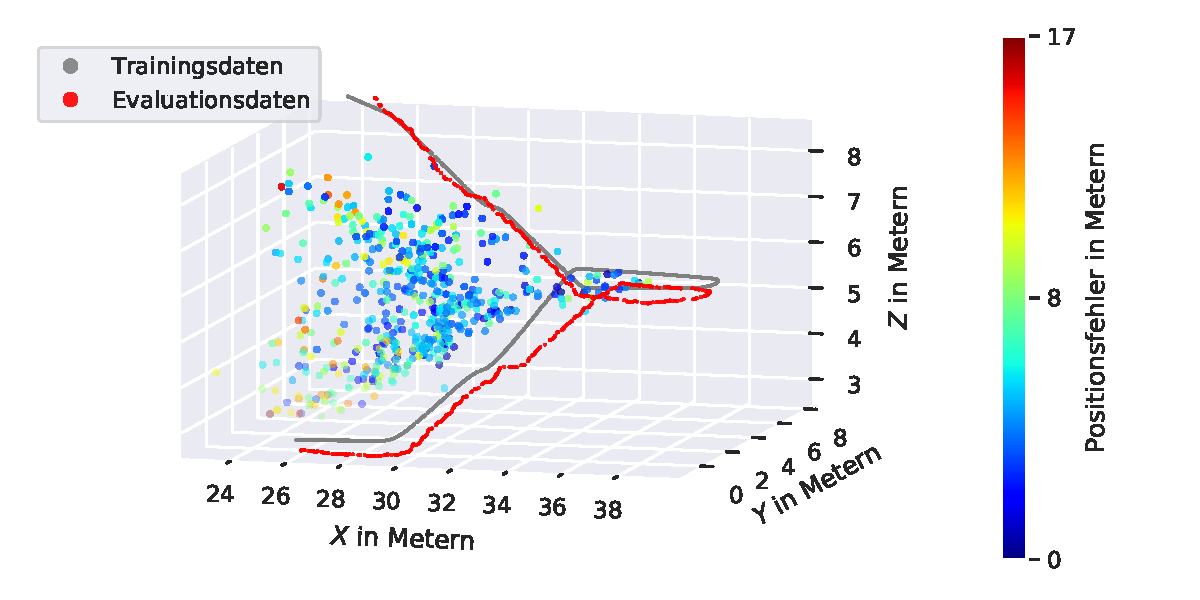
\includegraphics[width=1.0\linewidth]{images/results/hs_up/resultsfig_3.pdf} }\\
		\subcaption{} \label{subfig:hs_up_fig5} & \imagetop{ 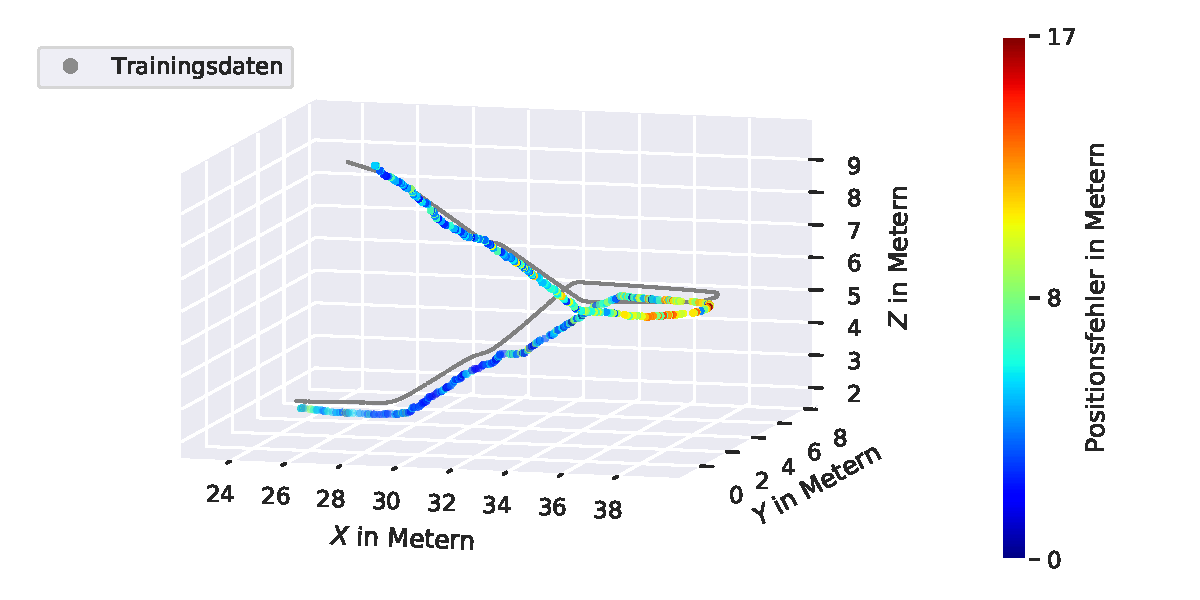
\includegraphics[width=1.0\linewidth]{images/results/hs_up/resultsfig_5.pdf} }\\
		\subcaption{} \label{subfig:hs_up_fig7} & \imagetop{ 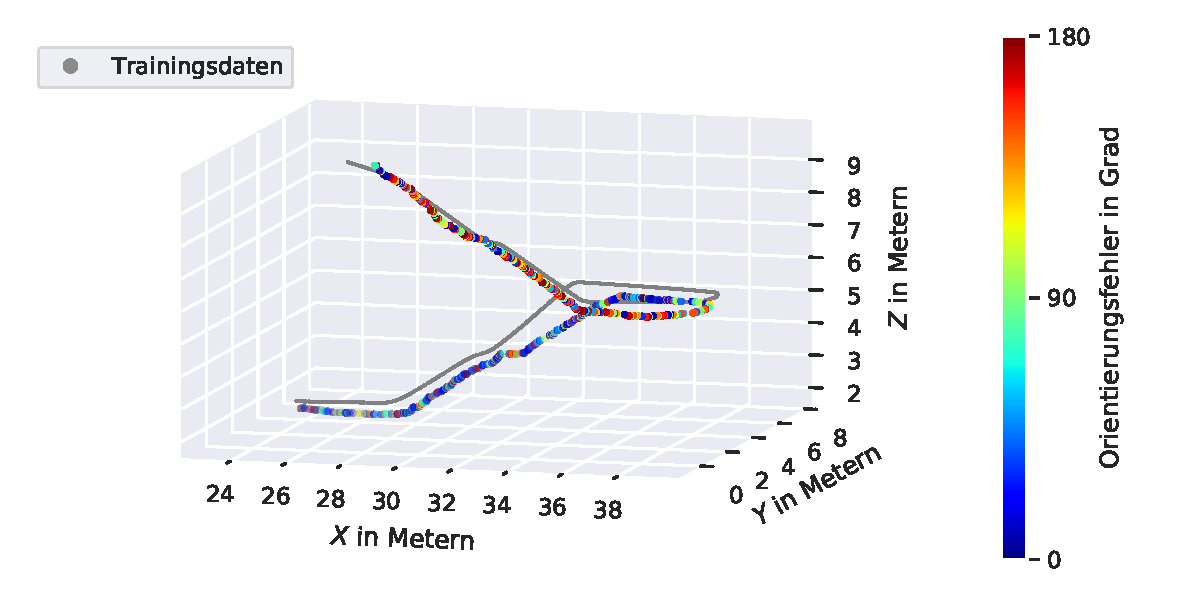
\includegraphics[width=1.0\linewidth]{images/results/hs_up/resultsfig_7.pdf} }\\
	\end{tabularx}
	\caption{Visualisierung der Evaluationsergebnisse der Strecke \textit{HS-stairs-up}. Die Evaluation folgte mit den Gradietenbildern der realen Daten auf dem mit \textit{grad-edge} trainierten Netzwerk. \subref{subfig:hs_up_fig3} illustriert die von dem KNN bestimmten Positionen auf der xy-Ebene. Der Positionsfehler in der xy-Ebene und der Orientierungsfehler auf der Gierachse der jeweiligen Evaluationsdaten werden in \subref{subfig:hs_up_fig5} und \subref{subfig:hs_up_fig7} dargestellt.} 
	\label{fig:result_hs_stairs_up}
\end{figure}


\subsubsection{HS-stairs-down}
\label{subsubsec:hs_stairs_down}
% Dies zeigt das Potenzial des Experimentes zur Pose Bestimmung mit Daten der gleichen Beschaffenheit auf der \textit{HS-stairs-down} Strecke.

Zuletzt wurde ein Experiment mit dem \textit{HS-stairs-down} Datensatz durchgeführt. Nur mit synthetischen Daten beim Trainieren und Evaluieren wurde eine Akkuratesse von 0.85$m$ in der Position und 7.50° in der Orientierung durch die \textit{grad-edge} Daten erzielt. Die Evaluierung mit den \textit{grad-real} Evaluationsdaten auf dem mit \textit{grad-cartoon} trainiertem Netzwerk führte zur einer Akkuratesse von 4.20$m$ in der Position und 47.83° in der Orientierung (vgl. Tab. \ref{tab:results_hs_stairs_down}). 

% Bei einem ca. $12m \times 12m \times 12m$ großen Zone ist eine Positionsgenauigkeit von 4.20$m$ sowie ein Orientierungsfehler von 47.83° unvollkommen für die Bestimmung der Pose auf der \textit{HS-stairs-down} Strecke. Abbildung \ref{fig:result_hs_stairs_down} visualisiert die Evaluationsergebnisse von dem mit \textit{grad-cartoon} trainiertem und \textit{grad-real} evaluiertem Netzwerk.


Das mit \textit{grad-cartoon} trainierte Netzwerk bestimmte die Positionen aller \textit{grad-real} Evaluationsdaten gleichermaßen wie im Unterabschnitt \ref{subsubsec:hs_stairs_up} zwischen dem unteren und oberen Treppenlauf (vgl. Abb. \ref{subfig:hs_down_fig3}). Deshalb waren hierbei genauso die größten Positionsfehler bei den Evaluationsdaten des Treppenabsatzes aufzufinden. Ebenso waren bei den Evaluationsdaten des unteren und oberen Treppenlaufes abwechselnd größere Positionsfehler zu erkennen. Diesmal wiesen die Evaluationsdaten des unteren Treppenlaufes häufiger einen größeren Positionsfehler auf (vgl. Abb. \ref{subfig:hs_down_fig5}). Im Vergleich zur \textit{HS-stairs-up} \ref{subsubsec:hs_stairs_up} ist in der Abbildung \ref{subfig:hs_down_fig7} entlang der Treppenläufe eine stärkere Abwechslung der Orientierungsfehler zu erkennen.

\begin{table}
	\centering
	\caption{Evaluationsergebnisse von der Strecke \textit{HS-stairs-down} (s. Abb. \ref{subfig:traj_hs-down}). Die Akkuratesse der mit den jeweiligen Trainingsdaten trainierten Netzwerken wird angegeben. Diese Netzwerke wurde mit den korrespondierenden synthetischen Evaluationsdaten und jeweils mit den realen Evaluationsdaten evaluiert.}
	\begin{tabularx}{1.0\textwidth}{X >{\RaggedRight}X >{\RaggedRight}X}
		\textbf{Netzwerk} \hspace{2cm} (Trainingsdatensatz) & \textbf{synthetische Daten} \hspace{2cm} (Position, Orientierung) & \textbf{reale Daten} \hspace{2cm} (Position, Orientierung)\\
		\hline
		\textit{grad-cartoon} & 0.91$m$, 8.01° & 4.20$m$, 47.83°\\
		\hline
		\textit{grad-edge} & 0.85$m$, 7.50° & 5.59$m$, 67.34°\\
		\hline
		\textit{grad-photoreal} & 1.02$m$, 8.57° & 5.25$m$, 32.70°\\
	\end{tabularx}
	\label{tab:results_hs_stairs_down}
\end{table}


\begin{figure}
	\setlength\extrarowheight{-15pt}
	\centering
	\begin{tabularx}{0.9\textwidth}{>{\centering\arraybackslash}p{0.05\textwidth} X}
		\subcaption{} \label{subfig:hs_down_fig3} & \imagetop{ 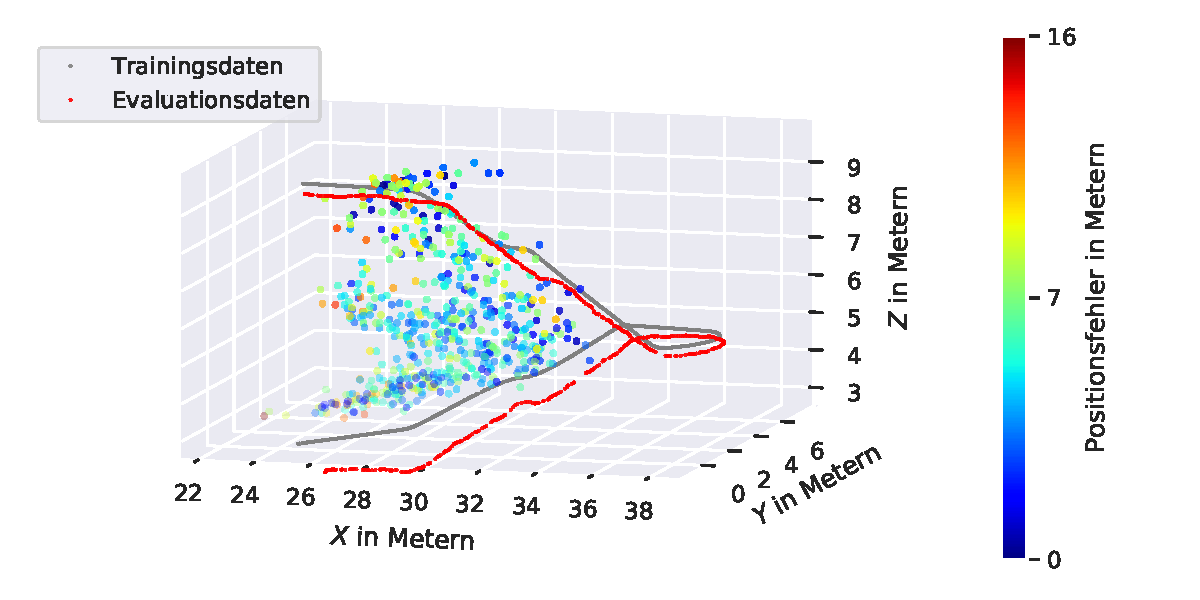
\includegraphics[width=1.0\linewidth]{images/results/hs_down/resultsfig_3.pdf} }\\
		\subcaption{} \label{subfig:hs_down_fig5} & \imagetop{ 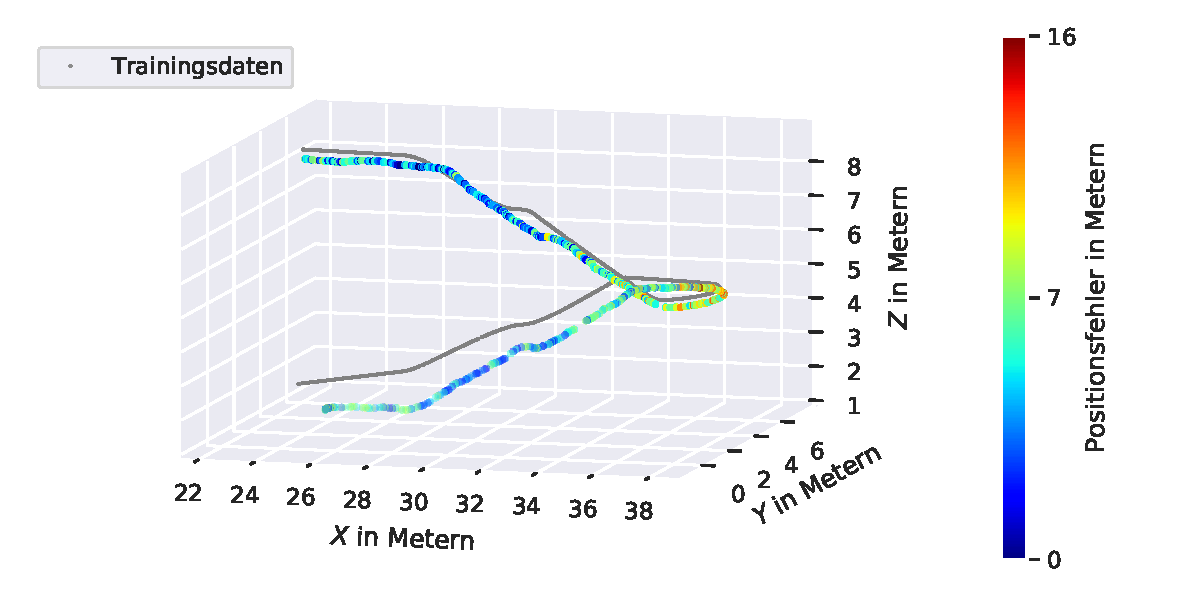
\includegraphics[width=1.0\linewidth]{images/results/hs_down/resultsfig_5.pdf} }\\
		\subcaption{} \label{subfig:hs_down_fig7} & \imagetop{ 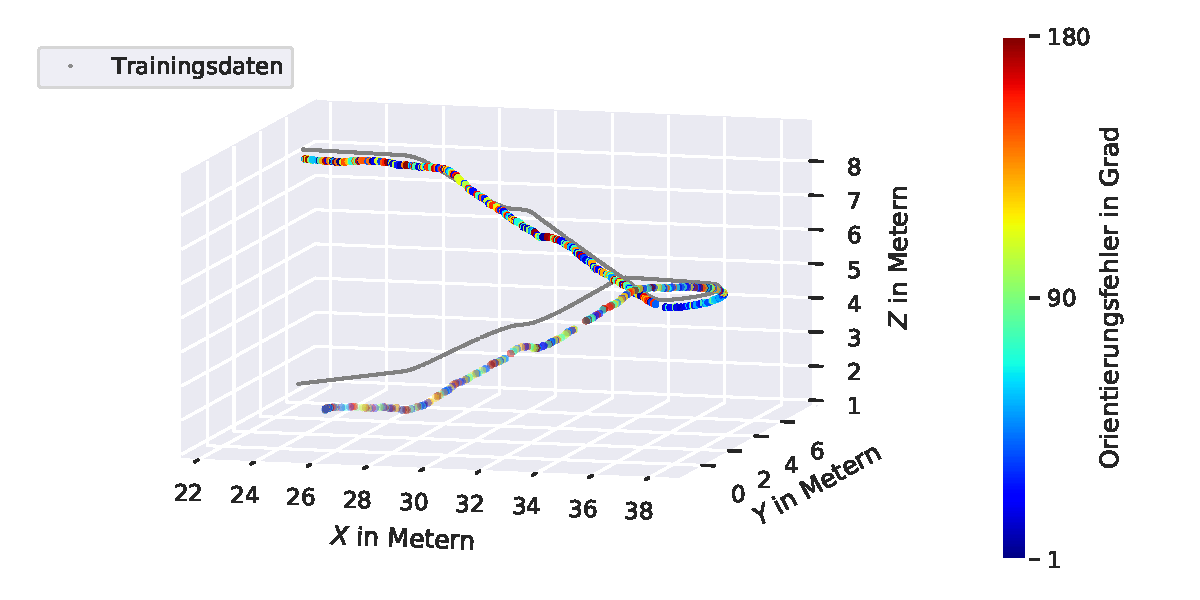
\includegraphics[width=1.0\linewidth]{images/results/hs_down/resultsfig_7.pdf} }\\
	\end{tabularx}
	\caption{Visualisierung der Evaluationsergebnisse der Strecke \textit{HS-stairs-down}. Die Evaluation folgte mit den Gradietenbildern der realen Daten auf dem mit \textit{grad-cartoon} trainierten Netzwerk. \subref{subfig:hs_down_fig3}  illustriert die von dem KNN bestimmten Positionen auf der xy-Ebene. Der Positionsfehler in der xy-Ebene und der Orientierungsfehler auf der Gierachse der jeweiligen Evaluationsdaten werden in \subref{subfig:hs_down_fig5} und \subref{subfig:hs_down_fig7} dargestellt.}
	\label{fig:result_hs_stairs_down}
\end{figure}





